\begin{figure}[t]
\centering
\subfigure[Impact of Increasing Passage Number]{
\begin{minipage}[t]{0.45\linewidth}
\centering
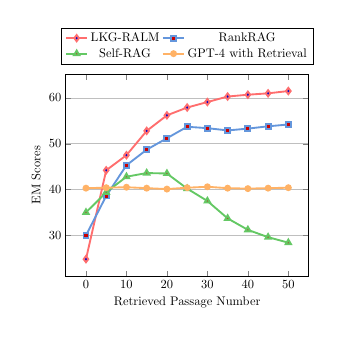
\begin{tikzpicture}[scale=0.45]
    \begin{axis}[
        xlabel=Retrieved Passage Number,
        ylabel=EM Scores,
        % y label style={at={(-0.0,0.5)}},
        ymajorgrids=true,
        font=\Large,
        legend style={at={(0.5,1.05)}, anchor=south, legend columns=2, draw=black, fill=white,align=left},font=\normalsize
    ]
        \addplot+[color={rgb,255:red,255;green,110;blue,110}, line width=1.5pt, mark=diamond*, mark size=2.5pt] coordinates {        
            (0,24.8)
            (5,44.2)
            (10,47.5)
            (15,52.8)
            (20,56.2)
            (25,57.9)
            (30,59.1)
            (35,60.3)
            (40,60.7)
            (45,61.0)
            (50,61.5)
        };
        \addlegendentry{LKG-RALM};
        \addplot+[color={rgb,255:red,100;green,150;blue,220}, line width=1.5pt, mark=square*, mark size=2pt] coordinates {
            (0,30.0)
            (5,38.6)
            (10,45.3)
            (15,48.7)
            (20,51.2)
            (25,53.7)
            (30,53.4)
            (35,52.9)
            (40,53.3)
            (45,53.8)
            (50,54.2)
        };
        \addlegendentry{RankRAG};
        \addplot+[color={rgb,255:red,100;green,200;blue,100}, line width=1.5pt, mark=triangle*, mark size=2.5pt] coordinates {
            (0,35.0)
            (5,39.4)
            (10,42.8)
            (15,43.6)
            (20,43.5)
            (25,40.2)
            (30,37.5)
            (35,33.7)
            (40,31.2)
            (45,29.6)
            (50,28.4)
        };
        \addlegendentry{Self-RAG};
        \addplot+[color=orange!60, line width=1.5pt, mark=*, mark size=2pt] coordinates {
            (0,40.3)
            (5,40.4)
            (10,40.5)
            (15,40.3)
            (20,40.1)
            (25,40.4)
            (30,40.6)
            (35,40.3)
            (40,40.2)
            (45,40.3)
            (50,40.4)
        };
        \addlegendentry{GPT-4 with Retrieval};
    \end{axis}
\end{tikzpicture}
\label{fig:q4-1}
\end{minipage}
}
\hfill
\subfigure[Impact of Irrelevant Passages]{
\begin{minipage}[t]{0.45\linewidth}
\centering
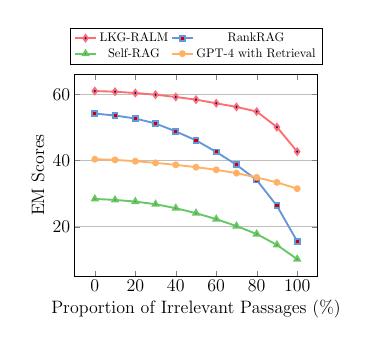
\begin{tikzpicture}[scale=0.45]
    \begin{axis}[
        xlabel=Proportion of Irrelevant Passages (\%),
        ylabel=EM Scores,
        % y label style={at={(-0.0,0.5)}},
        ymajorgrids=true,
        font=\Large,
        legend style={at={(0.5,1.05)}, anchor=south, legend columns=2, draw=black, fill=white,align=left,font=\normalsize},
    ]
        \addplot+[color={rgb,255:red,255;green,110;blue,110}, line width=1.5pt, mark=diamond*, mark size=2.5pt] coordinates {
            (0,61.0)
            (10,60.8)
            (20,60.4)
            (30,59.9)
            (40,59.2)
            (50,58.4)
            (60,57.3)
            (70,56.2)
            (80,54.8)
            (90,50.1)
            (100,42.7)
        };
        \addlegendentry{LKG-RALM};
        \addplot+[color={rgb,255:red,100;green,150;blue,220}, line width=1.5pt, mark=square*, mark size=2pt] coordinates {
            (0,54.2)
            (10,53.6)
            (20,52.7)
            (30,51.2)
            (40,48.8)
            (50,46.1)
            (60,42.6)
            (70,38.7)
            (80,34.1)
            (90,26.3)
            (100,15.6)
        };
        \addlegendentry{RankRAG};
        \addplot+[color={rgb,255:red,100;green,200;blue,100}, line width=1.5pt, mark=triangle*, mark size=2.5pt] coordinates {
            (0,28.4)
            (10,28.1)
            (20,27.6)
            (30,26.8)
            (40,25.6)
            (50,24.1)
            (60,22.3)
            (70,20.2)
            (80,17.8)
            (90,14.5)
            (100,10.2)
        };
        \addlegendentry{Self-RAG};
        \addplot+[color=orange!60, line width=1.5pt, mark=*, mark size=2pt] coordinates {
            (0,40.4)
            (10,40.2)
            (20,39.8)
            (30,39.3)
            (40,38.7)
            (50,38.0)
            (60,37.2)
            (70,36.2)
            (80,34.9)
            (90,33.4)
            (100,31.5)
        };
        \addlegendentry{GPT-4 with Retrieval};
    \end{axis}
\end{tikzpicture}
\label{fig:q4-2}
\end{minipage}
}
\caption{Robustness to the number of retrieved passages and the proportion of irrelevant passages.}
\label{fig:impact_passages}
\end{figure}